% Drawing 154/08-13 -- folder 154, batch 08, archive page 157 (PDF page 158).
% Transcription: à gauche, un grand dessin : trois droites numérotées $1$, $2$, $3$ (brune, noire, brun foncé) formant un triangle hachuré, orienté par une flèche de rotation ; en chacun des trois sommets, un point de couleur (bleu, vert, orange) entouré de deux arcs de la même couleur fléchés. À droite, le triangle dual : trois droites $1$, $2$, $3$ (bleu clair, orange, vert clair) aux sommets bruns, les arcs bruns et noirs fléchés, l'orientation $\omega'$. Au-dessous, deux croquis : une droite $1$ au point $2$, les vecteurs $\alpha$ (le long de la droite), $\beta$ (transverse) et la rotation $\omega$ ; une droite vert clair au point marqué, avec $\omega'$, $\beta'$, $\alpha'$
% Kind: three numbered lines forming a hatched oriented triangle with coloured vertices; the dual triangle; small frames. Method 2 (schematic redraw from the facsimile). Status: partial.
% Notes: Left, a large drawing: three lines numbered 1, 2, 3 (brown, black, dark brown) forming a hatched triangle, oriented by a rotation arrow; at each of the three vertices a coloured point (blue, green, orange) surrounded by two arrowed arcs of the same colour. To the right, the dual triangle (orange, yellow-green and grey-blue lines) with its vertices and a rotation arrow; below, small frames with the orientations alpha, beta, omega and a yellow line with omega'. Read from the page view; the pencilled text between is the transcription's.
% Coordinates: 1 unit = 1 mm = 1/100 of the crop width (bbox in page fractions: [0.132, 0.147, 0.764, 0.402]).
% Redrawn by Claude (claude-opus-5-5), issue #73, 2026-11-07; not checked by a human; not compiled (no TeX in the session).
% Rights: reproduces part of the work -- behind RENDER_TRANSCRIPTS, never published by itself.
\documentclass[tikz,border=3pt]{standalone}
\usepackage{amsmath,amssymb}
\usetikzlibrary{patterns,arrows.meta}
\tikzset{Or/.style={orange!90!black}, Ye/.style={yellow!80!orange}, Lg/.style={green!60!black!70}, Dg/.style={green!45!black}, Br/.style={brown!80!black}, Rd/.style={red!85!black}, Bl/.style={blue!70!black}, Gy/.style={black!40}, pencil/.style={black!45}, struck/.style={black!35}, mark/.style={circle,draw,inner sep=1.3pt}, pt/.style={circle,fill,inner sep=0.9pt}, opt/.style={circle,draw,fill=white,inner sep=1.1pt}}
\begin{document}
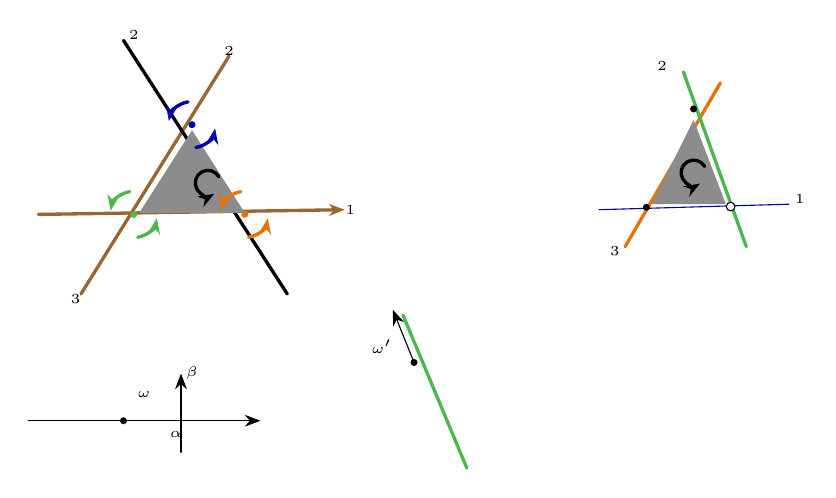
\begin{tikzpicture}[x=1mm,y=1mm,line cap=round,line join=round,font=\scriptsize]
\draw[Br,very thick,-{Stealth[length=2mm]}] (2,-24.8) -- (40.9,-24.2);
\draw[Br,very thick] (7.4,-34.9) -- (26.2,-4.7);
\draw[very thick] (12.8,-2.7) -- (33.6,-34.9);
\fill[pattern=north east lines,pencil] (14.8,-24.6) -- (21.5,-14.1) -- (28.2,-24.6) -- cycle;
\node[inner sep=1pt] at (41.6,-24.2) {\tiny $1$};
\node[inner sep=1pt] at (26.2,-4) {\tiny $2$};
\node[inner sep=1pt] at (6.7,-35.6) {\tiny $3$};
\node[inner sep=1pt] at (14.1,-2) {\tiny $2$};
\draw[-{Stealth[length=2mm]},very thick] (24.9,-20) arc[start angle=30, end angle=300, x radius=1.6, y radius=1.6];
\node[pt,Bl] at (21.5,-13.4) {};
\draw[Bl,very thick,-{Stealth[length=2mm]}] (21,-10.5) arc[start angle=100, end angle=170, x radius=3, y radius=3];
\draw[Bl,very thick,-{Stealth[length=2mm]}] (22,-16.3) arc[start angle=280, end angle=350, x radius=3, y radius=3];
\node[pt,Lg] at (14.1,-24.8) {};
\draw[Lg,very thick,-{Stealth[length=2mm]}] (13.6,-21.9) arc[start angle=100, end angle=170, x radius=3, y radius=3];
\draw[Lg,very thick,-{Stealth[length=2mm]}] (14.6,-27.7) arc[start angle=280, end angle=350, x radius=3, y radius=3];
\node[pt,Or] at (28.2,-24.8) {};
\draw[Or,very thick,-{Stealth[length=2mm]}] (27.7,-21.9) arc[start angle=100, end angle=170, x radius=3, y radius=3];
\draw[Or,very thick,-{Stealth[length=2mm]}] (28.7,-27.7) arc[start angle=280, end angle=350, x radius=3, y radius=3];
\draw[Or,very thick] (76.5,-28.9) -- (88.6,-8.1);
\draw[Lg,very thick] (83.9,-6.7) -- (91.9,-28.9);
\draw[Bl] (73.2,-24.2) -- (97.3,-23.5);
\node[pt] at (85.2,-11.4) {};
\node[pt] at (79.2,-23.9) {};
\node[opt] at (89.9,-23.8) {};
\fill[pattern=north east lines,pencil] (79.9,-23.5) -- (85.2,-12.8) -- (89.3,-23.5) -- cycle;
\draw[-{Stealth[length=2mm]},very thick] (86.6,-18.7) arc[start angle=30, end angle=300, x radius=1.6, y radius=1.6];
\node[inner sep=1pt] at (98.7,-22.8) {\tiny $1$};
\node[inner sep=1pt] at (81.2,-6) {\tiny $2$};
\node[inner sep=1pt] at (75.2,-29.5) {\tiny $3$};
\draw[-{Stealth[length=2mm]}] (0.7,-51) -- (30.2,-51);
\node[pt] at (12.8,-51) {};
\draw[-{Stealth[length=2mm]}] (20.1,-55) -- (20.1,-45);
\node[inner sep=1pt] at (15.4,-47.7) {\tiny $\omega$};
\node[inner sep=1pt] at (19.5,-52.8) {\tiny $\alpha$};
\node[inner sep=1pt] at (21.5,-45) {\tiny $\beta$};
\draw[Lg,very thick] (56.4,-57) -- (48.3,-37.6);
\node[pt] at (49.7,-43.6) {};
\draw[-{Stealth[length=2mm]}] (49.7,-43.6) -- (47,-36.9);
\node[inner sep=1pt] at (45.6,-41.6) {\tiny $\omega'$};
\end{tikzpicture}
\end{document}
